\chapter{Cassandra}

Esse trabalho ira utilizar o Cassandra como banco de dados para validação de sua hipótese. Como visto no capítulo 3, o Apache Cassandra, distribuição que sera utilizada, é um banco de dados orientado a colunas altamente disponível e distribuído em servidores constituídos de hardware de \enquote{prateleira} para gerenciamento de grande volumes de dados~\cite{lakshmancassandra}. Este capítulo tem como objetivo definir esse banco de dados, suas características, funcionamento, vantagens e desvantagens.

\section{Definição}
O Cassandra se originou em 2007 como um projeto do \emph{Facebook} para resolver um problema na busca da caixa de mensagens. A compania necessitava de um sistema com alta performance, confiabilidade, eficiência e que suportasse o contínuo crescimento da ferramenta~\cite{lakshmancassandra, cassandraguide}. 

O projeto foi desenvolvido por Jeff Hammerbacher, Avinash Lakshman, Karthik Ranganathan e Prashant Malik, tendo seu modelo de dados sofrido grande inspiração nos trabalhos anteriores do \emph{Amazon Dynamo}~\cite{dynamo} e do \emph{Google Bigtable}~\cite{bigtable}, e lançado em 2008 como um projeto \emph{open source}. Foi mantido e atualizado apenas pelo Facebook até 2009, quando foi comprado pela Apache~\cite{cassandraguide}, sendo utilizado atualmente por companias como \emph{Netflix}, \emph{Spotify} e até em agências governamentais, como a NASA~\cite{cassandracompanies}. 

O Apache Cassandra pode ser definido como um banco de dados orientado a colunas \emph{open source}, distribuído, descentralizado, elasticamente escalavel, altamente disponível, tolerante a falhas e variavelmente consistente~\cite{cassandraguide}. A seguir iremos analisar cada uma dessas características.

\subsection{Características}

\subsection*{Distribuído e Descentralizado}
O Cassandra é capaz de ser executado em múltiplas de forma transparente ao usuário, que o enxerga como um sistema unificado. Apesar de ser possível sua execução em um único nó, só é possível obter algum benefício com uma execução distribuída. Além do ganho de performance, a distributividade do sistema garante maior segurança devido à redundância de dados.

Diferente de outros bancos distribuidos que elegem nós como mestres e escravos, o Cassandra opera de forma descentralizada, o que significa que todos os nós são idênticos em sua forma de execução, sendo utilizados protocolos \emph{peer-to-peer} (par-a-par) e \emph{gossip} para manutenção e sincronia entre os nós. Essa descentralização garante que não exista apenas um ponto de falha, o que aumenta sua disponibilidade, e simplifica a operação do e manutenção do \emph{cluster}.

\subsection*{Elasticamente Escalável}
Escalabilidade é a propriedade que um sistema tem de atender um crescente número de requisições sem prejuízo de performance. Essa escalabilidade pode ser tanto vertical quanto horizontal. Na escalabilidade vertical o hardware já utilizado no sistema é melhorado, enquanto na escalabilidade horizontal novos máquinas são adicionadas à arquitetura, havendo a divisão da carga do sistema.

O Cassandra possui escalabilidade horizontal elástica, o que significa que sua arquitetura pode escalar tanto para cima quanto para baixo. Na necessidade de uma melhora do desempenho da aplicação, novas máquinas podem ser adicionadas, e o Cassandra se encarrega de fazer a distribuição dos dados de forma transparente, sem necessidade de configurações adicionais ou reiniciamento do sistema. Da mesma forma, em caso de necessidade, máquinas podem ser retiradas do \emph{cluster} sem prejuizo ao todo, devido ao rebalanceamento automático.

\subsection*{Altamente disponível e Tolerante a falhas}
A disponibilidade de um sistema é medida de acordo com sua capacidade de responder a requisições. Computadores, e especialmente sistemas distribuídos em rede, estão sujeitos a falhas, que em geral só podem ser contornadas por meio de sistemas redundantes.

Devido a replicação e redundância de dados e a sua capacidade de substituição de nós indisponíveis, o Cassandra pode ser definido como um sistema altamente disponível e tolerante à falhas em suas máquinas.

\subsection*{Variavelmente Consistente}
A consistência de uma aplicação diz respeito à sua capacidade de retornar o valor mais atual em uma requisição.

Como visto no Teorema CAP\ref{sec:cap}, não é possível a um sistema ser totalmente conscistente, disponível e tolerante a falhas. 

O Cassandra é por vezes definido como \enquote{eventualmente consistente}, por trocar parte de sua consistência por alta disponibilidade. Essa definição, porém, não é totalmente correta, e um termo melhor para defini-lo é \enquote{variavelmente consistente} (\emph{tuneably consistent}), podendo essa sua consistência ser ajustada de acordo com o tipo de aplicação.

\section{Modelo de Dados}

Um banco de dados Cassandra consiste em um \emph{keyspace} contendo famílias de colunas, que por sua vez definem um conjunto de linhas que englobam várias colunas. Essa disposição de dados é bastante semelhante ao que foi proposto pelo Bigtable~\cite{lakshmancassandra, bigtable}. Seu modelo de dados pode ser visto como um mapa multidimensional indexado por uma chave, se assemelhando aos modelos de chave-valor e orientados à colunas. A seguir veremos em detalhes cada um desses conceitos.

A figura \ref{fig:cassandradm} ilustra de forma resumida o modelo de dados do Cassandra, contendo um \emph{keyspace} e seus componentes. 

\begin{figure}[!htb]
\centering
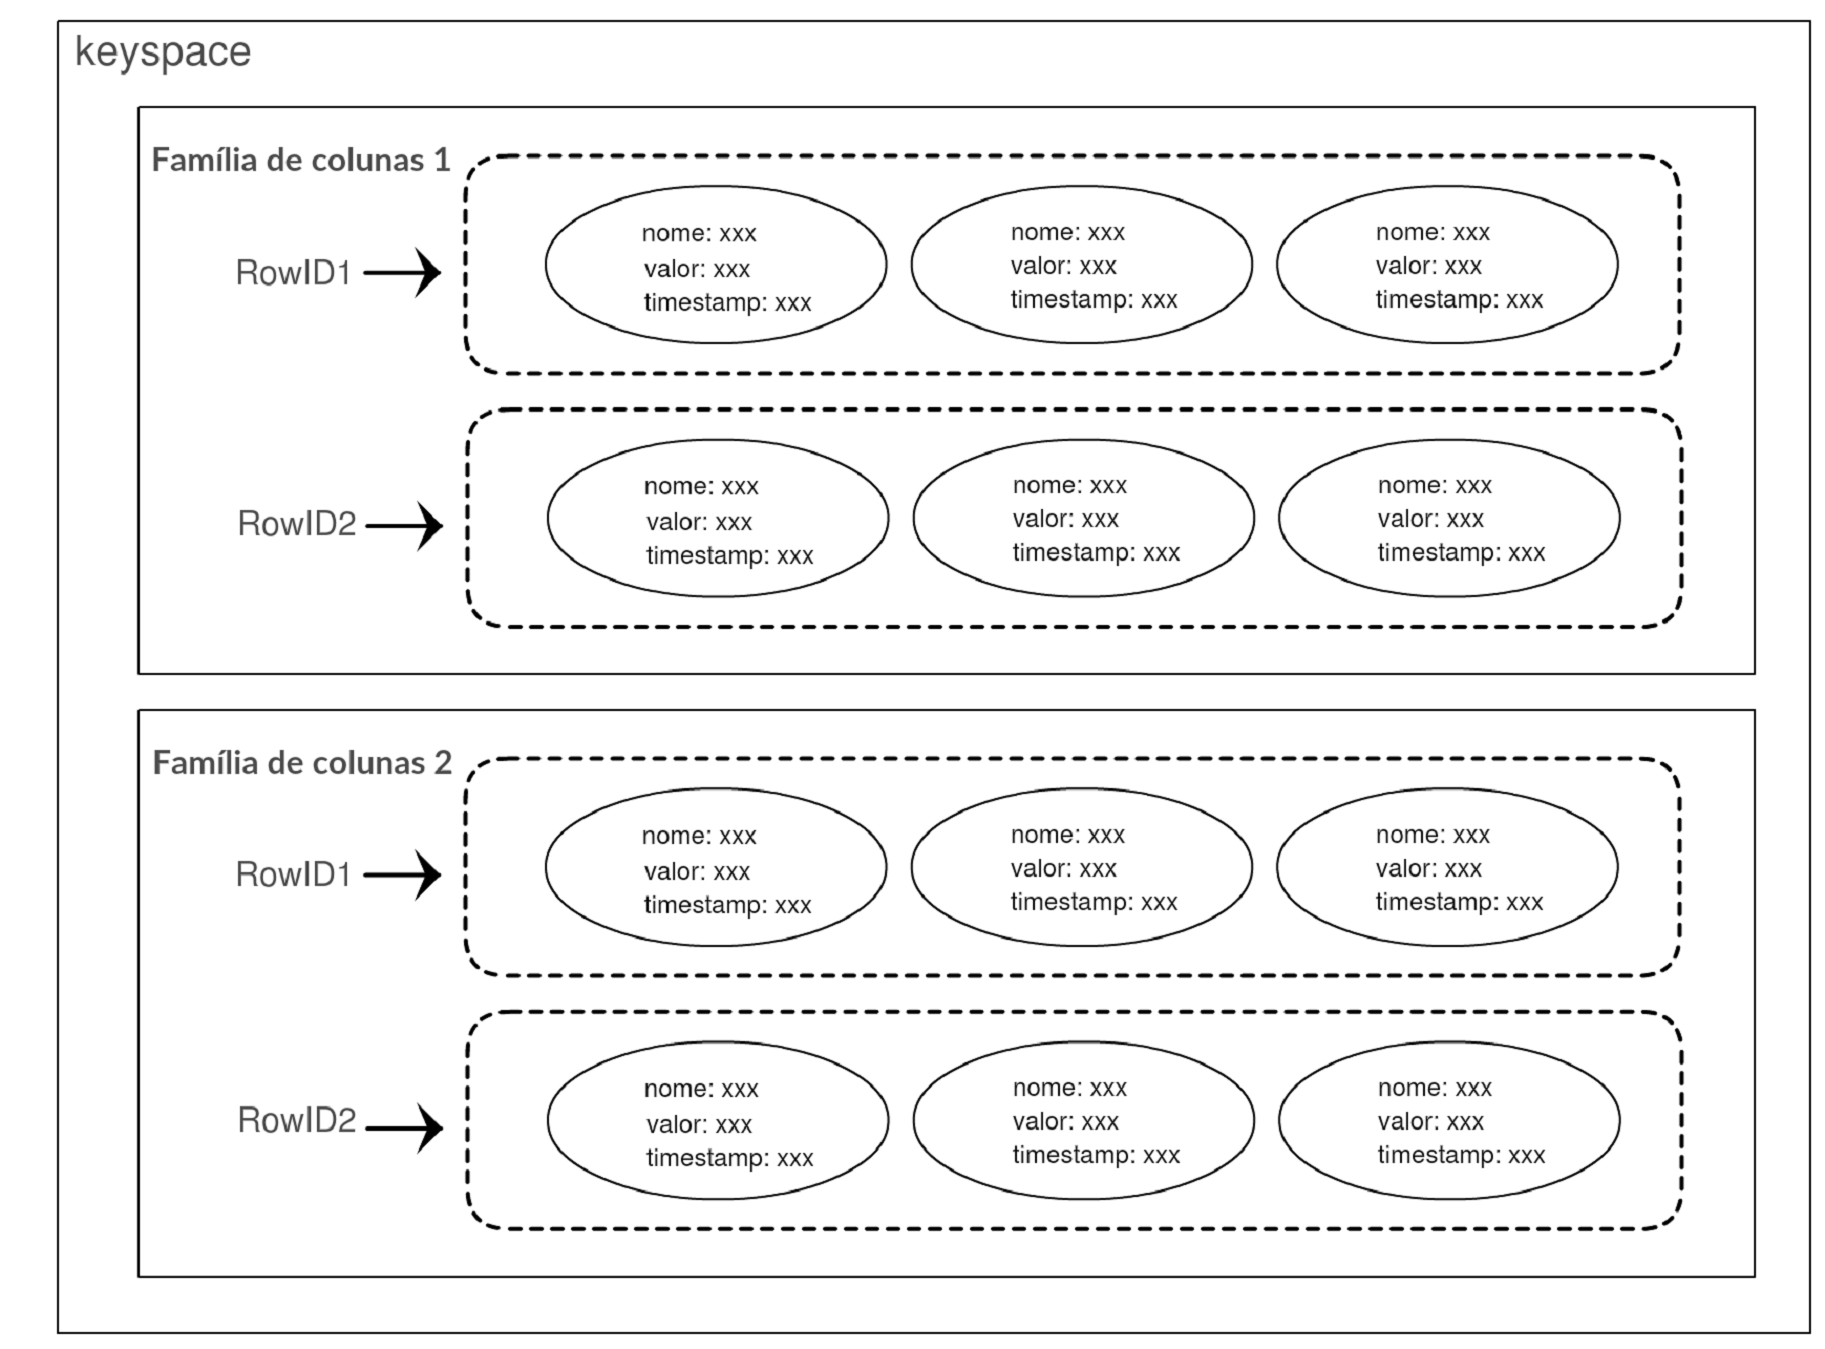
\includegraphics[width=1.1\textwidth]{figuras/cassandradatamodel.png}
\caption{Modelo de dados do Cassandra. Adaptado de ~\cite{ibmcassandra}}
\label{fig:cassandradm}
\end{figure}

\subsection*{\emph{Keyspace}}
Um \emph{keyspace} define o agrupamento de dados mais externo no Cassandra, podendo ser correspondido a um banco de um SGBD relacional. Um \emph{keyspace} define um nome e uma série de atributos que definem o seu comportamento. 
Atributos do \emph{keyspace} incluem~\cite{cassandraguide}:
\begin{itemize}
\item \textbf{Fator de replicação} diz respeito ao número de nós que armazenarão uma réplica de cada linha de dados. O fator de replicação tem forte influencia no balanço entre performance e consistência do banco de dados.
\item \textbf{Estratégia de replicação} se refere a como as réplicas (ou cópias) de um dado serão posicionados no anel do \emph{cluster}. Diversas estratégias de replicação estão disponíveis no Cassandra.
\item \textbf{Famílias de colunas} pode ser visto como o análogo às tabelas de um modelo relacional, da mesma forma que o \emph{keyspace} é o análogo do banco.  Uma família de colunas é um agrupamento para uma coleção de linhas, onde cada linha contém colunas ordenadas.
\end{itemize}



\subsection*{Colunas e famílias de colunas}
Uma família de colunas (ou tabela) no Cassandra é um mapa multidimensional indexado por uma chave. Essa chave é uma \emph{string} sem restrição de tamanho, mas que em geral varia de 16 a 36 \emph{bytes}. O valor desse mapeamento consiste em uma família de colunas, um agrupamento para uma coleção ordenadas de linhas, que por sua vez é uma coleção ordenada de colunas ~\cite{lakshmancassandra, cassandraguide}.

Uma família de colunas possui dois atributos: um nome e um comparador. O nome identifica a coluna para realização de consultas, enquanto o comparador indica como as colunas serão ordenadas ao serem retornadas em uma consultas, podendo ser \emph{long}, \emph{byte}, UTF8, etc~\cite{cassandraguide}.

O modelo de família de colunas se diferencia do modelo relacional por ser o que é chamado comumente de \emph{livre de esquema} (\emph{schema free}) . É possível realizar a inserção, remoção ou alteração de qualquer coluna ou família de colunas a qualquer momento, ficando as aplicações clientes do banco encarregadas de interpretar e manipular o novo modelo de dados. 

Ao se inserir um novo dado em uma família de colunas do Cassandra são especificados valores para uma ou mais colunas. O conjunto de valores é chamado de linha, e é identificado unicamente por uma chave primária ou chave de linha. Uma linha não precisa possuir dados para todas colunas presentes na família de colunas à que ela pertence, sendo o espaço alocado apenas para as colunas presentes nessa linha. Isso gera tanto uma economia de espaço quanto uma melhora de performance em relação a um banco relacional, que precisa preencher com valores nulos colunas não utilizadas.

Uma coluna é a unidade básica de armazenamento do Cassandra, e é constituida por um nome, um valor e um \emph{timestamp}. Se difere do conceito de colunas de bancos relacionais pois durante a criação do banco não é necessário a criação de colunas, e sim apenas famílias de colunas. A criação de colunas ocorre apenas durante a inserção de dados no banco e suas colunas correspondentes~\cite{cassandraguide}.

\section{Arquitetura}

O Cassandra foi projetado para lidar com grandes massas de dados distribuídas em vários nós sem ponto único de falha, pensado no fato de que tanto um sistema quanto componentes de hardware podem falhar.
A arquitetura Cassandra combate o problema de falhas ao empregar uma distribuição par-a-par (\emph{peer-to-peer}) entre nós homogêneos, com dados distribuidos entre todos os nós de um \emph{cluster}~\cite{cassandradocs}. 

Cada nó frequentemente troca informações de estado sobre ele mesmo e outros nós do cluster utilizando um  protocolo par-a-par \emph{gossip}. Um \emph{commit log} sequencial em cada nó armazena atividades de escrita de dados para garantir durabilidade. Esses dados são então indexados e escritos em uma estrutura em memória RAM chamada \emph{memtable}. Sempre que a \emph{memtable} é completamente preenchida, os dados são escritos em disco em um arquivo \emph{SSTable}. Uma \emph{SSTable} é um arquivo imutável, onde os dados são apenas inseridos ao final do arquivo. Os arquivos \emph{SSTable} são então particionados e replicados no cluster, o que garante a redundância dos dados. Periodicamente, as \emph{SSTables} são compactadas e dados obsoletos são descartados, além disso a consistencia do \emph{cluster} é mantida por meio de mecanismos de reparo~\cite{cassandradocs}.

Consultas no Cassandra podem ser realizadas por meio da linguagem \emph{CQL}, que possui sintax próxima a do \emph{SQL} e trabalha com dados de tabelas. Operações de leitura e escrita podem ser realizados em qualquer nó do \emph{cluster}, devido à característica de homogeneidade entre eles. Ao realizar uma conexão com um cliente, o nó atua como coordenador dessa operação, servindo de ponte entre a aplicação e os nós que possuem o dado requisitado~\cite{cassandradocs}e. 